\documentclass[letterpaper,12pt,fleqn]{article}
\usepackage{matharticle}
\usepackage{siunitx}
\usepackage{tikz}
\pagestyle{plain}
\begin{document}

\begin{center}
  \large
  Math-19 Section 1

  \Large
  Homework \#2 Solutions
\end{center}

\subsection*{Problems}

\begin{enumerate}
\item A man stands atop a \SI{256}{ft} cliff with a  ball.  Recall that the equation of motion that we presented in
  class is given by:
  \[h=h_0+v_0t-16t^2\]
  \begin{enumerate}
  \item How long does it take for the ball to hit the ground if he simply releases the ball?
    \begin{gather*}
      0=256-16t^2 \\
      16t^2=256 \\
      t^2=16 \\
      t=\pm4
    \end{gather*}
    We only need the positive solution here, so:
    \[t=\SI{4}{s}\]
    Note that the negative solution represents the ball being thrown upward from the ground such that the ball
    stops at the top of the cliff.

  \item How long does it take for the ball to hit the ground if he throws the ball up with a velocity of \SI{16}{ft/s}?
    \begin{gather*}
      0=256+16t-16t^2 \\
      16t^2-16t-256=0 \\
      t^2-t-16=0 \\
      t^2-t=16 \\
      t^2-t+\frac{1}{4}=16+\frac{1}{4} \\
      \left(t-\frac{1}{2}\right)^2=\frac{65}{4} \\
      t-\frac{1}{2}=\pm\frac{\sqrt{65}}{2} \\
      t=\frac{1\pm\sqrt{65}}{2} \\
      t=-3.5,4.5
    \end{gather*}
    We only need the positive solution here, so:
    \[t=\SI{4.5}{s}\]
    Note that the negative solution represents the ball being thrown upward from the ground such that the ball is
    traveling at \SI{16}{ft/s} when it passes the top of the cliff.

  \item How long does it take for the ball to hit the ground if he throws the ball down with a velocity of
    \SI{16}{ft/s}? (Hint: no additional calculations are needed).

    We obtained this solution in the previous problem:
    \[t=\SI{3.5}{s}\]

  \item Assume that a lady is standing on the ground below the cliff and throws a ball up so that it passed the man
    on the cliff at a velocity of \SI{16}{ft/s}.  How long would it be before the ball hits the ground? (Hint: you
    already have all the information that you need).

    This is simply the sum of the times from the previous problems:
    \[t=4.5+3.5=\SI{8}{s}\]
  \end{enumerate}

\item You are a product manager at an electronics firm in charge of a proposed new line of 25-inch monitors (i.e.,
  the length of the diagonal across the screen is 25 inches):

  \begin{tikzpicture}
    \draw (0,0) rectangle (5,3);
    \draw [dashed] (0,0) -- (5,3);
    \node at (2.5,2.0) {25''};
    \node [above] at (2.5,0) {$\ell$};
    \node [right] at (0,1.5) {$w$};
  \end{tikzpicture}

  You realize that the most appealing ratio for the dimensions of the screen would follow the golden ratio:
  \[\frac{\ell}{w}=\frac{1+\sqrt{5}}{2}\approx1.6=\frac{8}{5}\]

  \begin{enumerate}
  \item Using the estimate of $8/5$, determine the dimensions ($\ell\times w$) for the new monitor. Round each
    dimension to two decimal places.

    Let the length \(w\) be the key variable.  Then, using the stated golden ratio constraint, we have:
    \[\ell=\frac{8}{5}w\]
    Now, using the Pythagorean Theorem:
    \begin{gather*}
      w^2+\left(\frac{8}{5}w\right)^2=25^2 \\
      w^2+\frac{64}{25}w^2=625 \\
      \frac{89}{25}w^2=625 \\
      w^2=\frac{15625}{89} \\
      w=\pm\sqrt{\frac{15625}{89}} \\
      w=\pm13.25
    \end{gather*}
    And so \(w=\SI{13.25}{in}\).  Now, using the golden ratio to find \(\ell\):
    \[\ell=\frac{8}{5}(13.25)=\SI{21.20}{in}\]
    Therefore, the desired dimensions are:
    \[\SI{13.25}{in}\times\SI{21.20}{in}\]
    
  \item There needs to be an equal amount of casing around the edges of the screen.  The packaging department
    would like the monitor and casing to have a total area of 400 square inches.

    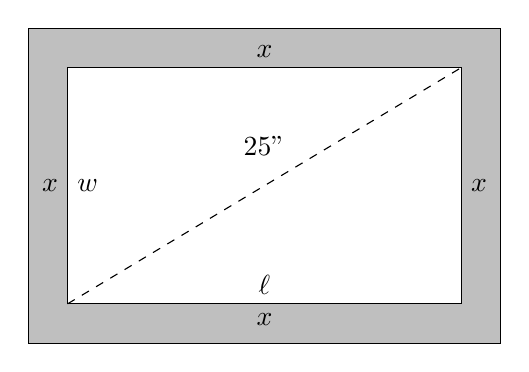
\begin{tikzpicture}
      \draw [fill=lightgray] (-0.5,-0.5) rectangle (5.5,3.5);
      \draw [fill=white] (0,0) rectangle (5,3);
      \draw [dashed] (0,0) -- (5,3);
      \node at (2.5,2.0) {25''};
      \node [above] at (2.5,0) {$\ell$};
      \node [right] at (0,1.5) {$w$};
      \node [above] at (2.5,3) {$x$};
      \node [below] at (2.5,0) {$x$};
      \node [left] at (0,1.5) {$x$};
      \node [right] at (5,1.5) {$x$};
    \end{tikzpicture}

    Determine the width of the casing ($x$) around the screen. Round your answer to
    two decimal places.
    \begin{gather*}
      (2x+w)(2x+\ell)=400 \\
      (2x+13.25)(2x+21.20)=400 \\
      4x^2+68.9x+280.9=400 \\
      4x^2+68.9x-119.1=0 \\
      x=\frac{-68.9\pm\sqrt{68.9^2-4(4)(-119.1)}}{2(4)} \\
      x=-18.80,1.58
    \end{gather*}
    Therefore, the padding should have a thickness of \SI{1.58}{in}.
  \end{enumerate}
\end{enumerate}

\end{document}
